Zum Überprüfen der Funktionalität haben wir eine Testengine entworfen. Die Klasse \emph{FeatureTest} bietet mit der Funktion \mintinline{java}{boolean testAllFeatures()} die Funktionalität aller beschriebenen Funktionalitäten zu überprüfen.

Um eine automatische Funktionsüberprüfung nach dem kompilieren zu erreichen, wurde die Klasse \mintinline{java}{RoboterWelt} erweitert, damit Sie den Test starten kann. Im Prinzip des OOP wurden jedoch alle Tests in einer seperaten Klasse durchgeführt.

Die Klasse \mintinline{java}{FeatureTest} bietet das Grundgerüst für die Testengine. Hier sind die Methoden zu Hause, die reflexiv auf Robby zugreifen, um die Rückgabewerte seiner Methoden zu überprüfen oder Felder auszulesen.

In der \mintinline{java}{FeatureTest} erweiternden Klasse \mintinline{java}{RobbyTest} sind die unten beschriebenen Testabläufe implementiert. Die volle Umsetzung aller im Lastenheft angeforderten Funktionen ist gelungen und wird zu Beginn jedes Programms mit einem Testlog, der bspw. in Abbildung~\ref{img:testlog} zu sehen ist, bestätigt.

\begin{figure}
\centering
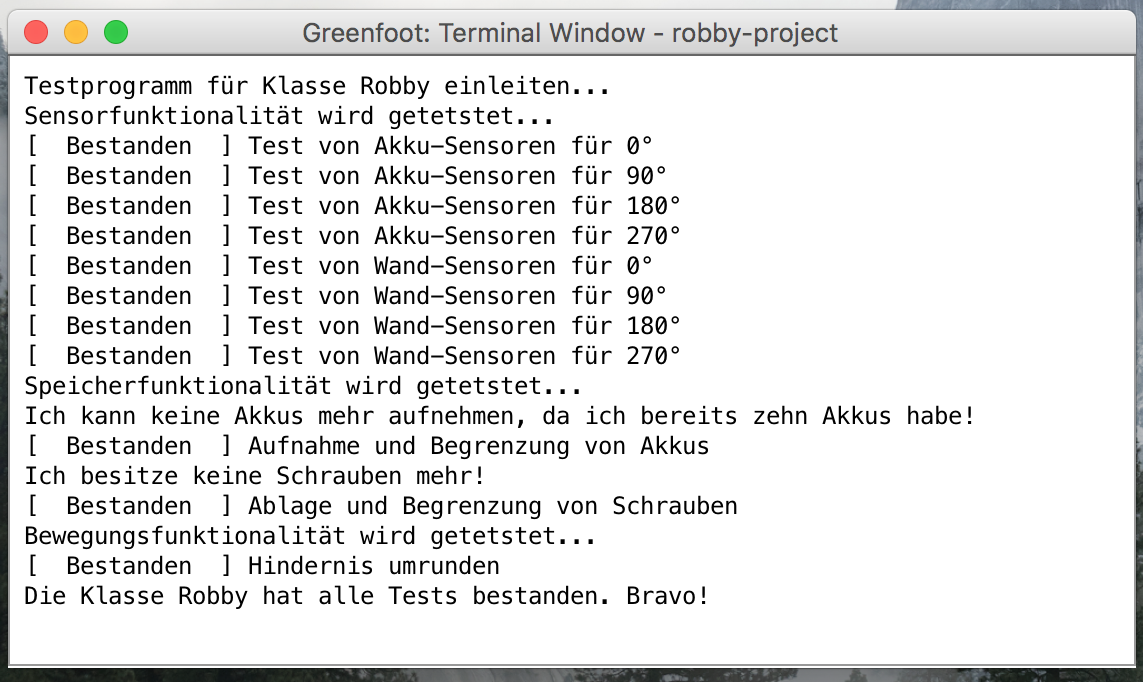
\includegraphics[width=\linewidth]{img/testlog}
\caption{Erfolgreicher Testlog nach dem Kompilieren der Klassen. }
\label{img:testlog}
\end{figure}

\subsection{Sensorik}
Robbys Sensorfunktionen für Akkus und Wände, die im Rahmen dieses Projekts erweitert wurden, sollen die jeweiligen Spielfiguren positiv, sowie negativ nachweisen können. Falsch positive und falsch negative Ergenisse müssen ausgeschlossen werden. Jede Funktion muss außerdem in unterschiedlichen Blickrichtungen getestet werden, um Zufallstreffer auszuschließen.

Im Gegensatz zur Implementierung der Funktionen in Robby müssen die Testfunktionen wasserdicht sein. Deduktive mathematische Beweise werden daher durch das ausprobieren jedes möglichen Falls in jeder Ausgangssituation getestet.

\subsubsection*{Testablauf}
Robby wird in Schleifen durch die verschiedenen Situationen/Winkel iteriert. Es wird für jeden Blickwinkel ($0^\circ, 90^\circ, 180^\circ$ und $270^\circ$) überprüft, ob die zuständige Funktion erkennt, dass kein Objekt neben Robby liegt und dass sich nach dem Einfügen des gesuchten Objekts neben Robby der Test positiv ausfällt. Die Objekte werden danach wieder aufgeräumt und aus der Welt entfernt. 

\subsubsection*{Situationen: }
Drehungen um $0^\circ, 90^\circ, 180^\circ$ und $270^\circ$
